\documentclass[]{article}
\usepackage{ctex}
\usepackage{graphicx}

%opening
\title{编译原理作业2}
\author{20152100121林伟业}
\date{}

\begin{document}

\maketitle

\section{实验内容}

设计一个应用软件,以实现将正则表达式-->NFA--->DFA-->DFA最小化---词法分析程序

\section{实验要求}

\begin{enumerate}
\item   要提供一个源程序编辑界面,让用户输入正则表达式(可保存、打开源程序)
\item   需要提供窗口以便用户可以查看转换得到的NFA(用状态转换表呈现即可)
\item   需要提供窗口以便用户可以查看转换得到的DFA(用状态转换表呈现即可)
\item   需要提供窗口以便用户可以查看转换得到的最小化DFA(用状态转换表呈现即可)
\item   需要提供窗口以便用户可以查看转换得到的词法分析程序(该分析程序需要用C语言
\item   应该书写完善的软件文档
\end{enumerate}

\section{程序说明}

实验使用编程语言:Python。主要文件NFA.py、DFA.py。程序运行:python DFA.py -s $"(a|b)^*abb"$。程序输出NFA,DFA,最小化的DFA,词法分析程序。

\section{类和函数说明}
NFA.py 文件
\subsection{类Condition}
保存NFA一个节点开始和结束状态的类

\subsection{类Node}
保存一个NFA机器的类,包含有开始结束状态和转移字符

\subsection{类Reg\_To\_NFA}
实现正则表达式转NFA。

思路:对正则表达式做开始前的处理,加入\&连接运算符,把读到的一个字符a到z,作为一个NFA机器添加到队列里,读取到的运算符保存到opt\_list队列里,运算符队列不为空的时候,取出运算符做相应的操作。连接运算符:在NFA机器队列里拿出2个,合并为一台机器后再加入到NFA的队列。闭包运算符:在状态队列里保存着最新添加到NFA队列里机器的开始和结束状态,读取到闭包运算符就从状态队列里拿出最新的2个状态,做闭包运算。或运算:在NFA队列里拿出两太机器,加入新的开始和结束状态,还有4条边,把合并后的机器重新加入和NFA队列。括号运算:把括号里的表达式拿出来,递归处理。

主要函数:
\begin{enumerate}
	\item def return\_NFA\_condition(self)  返回NFA的开始和结束状态
	\item def pre\_string(self):  正则表达式预处理函数,主要在两个字符之间加入\&连接运算符,方便处理
	\item def print\_NFA(self)  输出NFA
	\item def add\_to\_NFA(self, start\_condition, ch, end\_condition)  添加一个NFA机器
	\item def add\_to\_condition\_list(self, start\_condition, end\_condition)  添加一个NFA的开始和结束状态
	\item   def check\_oper(self)  检测运算符\&|()*,不同运算符分别处理。
	\item   def get\_one\_char(self)  获取正则表达式的一个字符,并返回
	\item   def to\_NFA(self, string)  主要函数,正则表达式转NFA
\end{enumerate}
DFA.py 文件

\subsection{类Node}
保存DFA机器状态,有开始,结束状态和转移字符

\subsection{类NFA\_To\_DFA}
实现NFA转DFA。
实现思路:将保存NFA机器的列表转变存储结构,方便DFA的状态转移遍厉。使用2个列表start\_map和end\_map。0->a->1,保存为 start\_map[0]=a,end\_map[0]=1,2->b->3,保存为start\_map[2]=b,end\_map[2]=3,如此类推。首先是找到包含开始状态和经过*转换的所有状态,作为DFA的第一个状态A。从A出发遍厉正则表达式的字母表,转换出其他状态BCD...

主要函数:
\begin{enumerate}
	\item  def pre\_oper(self)  将NFA转化成两个列表
	\item  def get\_alp\_from\_string(self)  获取正则表达式的字母表
	\item  def move(self, start, ch)  从开始状态start经过字符ch转移,返回结束状态列表
	\item  def add\_DFA\_list(self, start, ch, end)  添加一个DFA机器到列表,开始状态,结束状态,转移字符
	\item  def print\_DFA(self)  输出DFA
	\item  def make\_condition\_set(self)  主要算法,子集构造法
\end{enumerate}
~\\\
~\\\
\section{程序运行截图}
测试正则表达式(a|b)*abb

\begin{figure}[h]
	\centering
	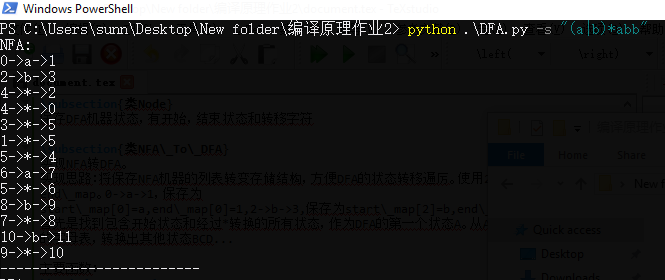
\includegraphics[width = 1\textwidth]{1.PNG}
	\caption{NFA}
\end{figure}

\begin{figure}[h]
	\centering
	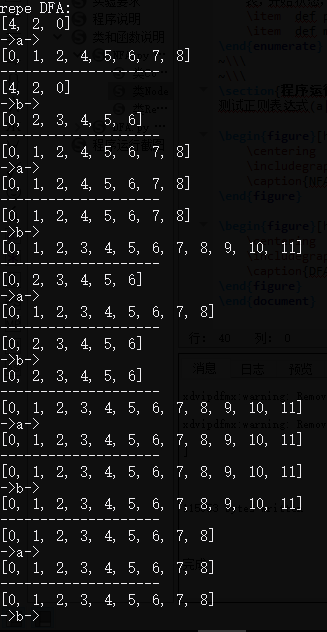
\includegraphics[width = 0.8\textwidth]{2.PNG}
	\caption{DFA}
\end{figure}
\end{document}
